%%%%%%%%%%%%%%%%%%%%%%%%%%%%%%%%%%%%%%%%%%%%%%%%%%%%%%%
% Based on the MatPlotLib and Random Cheat Sheet
% Edited by Michelle Cristina de Sousa Baltazar
%
% http://matplotlib.org/api/pyplot_summary.html
% http://matplotlib.org/users/pyplot_tutorial.html
%
%%%%%%%%%%%%%%%%%%%%%%%%%%%%%%%%%%%%%%%%%%%%%%%%%%%%%%%

\documentclass{article}
\usepackage[landscape]{geometry}
\usepackage{url}
\usepackage{multicol}
\usepackage{amsmath}
\usepackage{amsfonts}
\usepackage{amsmath,amssymb}

\usepackage{colortbl}
\usepackage{xcolor}
\usepackage{mathtools}
\usepackage{amsmath,amssymb}
\usepackage{enumitem}

\usepackage[english]{babel}
\usepackage[utf8]{inputenc}

\advance\topmargin-.8in
\advance\textheight3in
\advance\textwidth3in
\advance\oddsidemargin-1.5in
\advance\evensidemargin-1.5in
\parindent0pt
\parskip2pt
\newcommand{\hr}{\centerline{\rule{3.5in}{1pt}}}

\DeclareMathOperator{\argmin}{argmin}
\DeclareMathOperator{\argmax}{argmax}
\DeclareUnicodeCharacter{2716}{✖}
\begin{document}

\begin{center}{\huge{\textbf{Support Vector Machines cheatsheet}}}\\
	{\large By Jérémy Fix, Hervé Frezza-Buet}
\end{center}
\begin{multicols*}{3}

\section*{Kernels}
The separator reads
\begin{align*}
	h_{w, b}(x) = \sum_i w_i k(x_i, x) + b
\end{align*}
\begin{center}
	\begin{tabular}{lp{5cm} c}
		\textit{Linear} & $k(x, x') = <x, x'>$ \\
		\hline
		\textit{RBF} & $k_\sigma(x, x') = \exp(-\frac{\|x - x'\|^2}{2\sigma^2})$ \\ 
		\hline
		\textit{Polynomial} & $k_{\gamma, c, d}(x, x') = (\gamma <x, x'> + c)^d$ \\ 
	\end{tabular}
\end{center}

\section*{Classification SVM : C-SVC}
Primal optimization problem:
\begin{flalign*}
	\underset{w, b \xi}{\argmin}& \frac{1}{2} \|w\|^2 + C \mathbf{1}^T \xi\\
	\mbox{subject to}& \left\{\begin{array}{ll} 
			y_i h_{w, b}(x_i) \geq 1 - \xi_i &,  \forall (x_i, y_i) \in S \\
			\xi_i \geq 0&, \forall i
	\end{array}\right.
		\end{flalign*} 
		Dual optimization problem:
		\begin{flalign*}
			\underset{\alpha}{\argmin}& \frac{1}{2} \alpha^T Q \alpha - \mathbf{1}^T \alpha\\
			\mbox{subject to}& \left\{\begin{array}{ll} 
					y^T \alpha = 0\\
					0 \leq \alpha_i \leq C, \forall i
			\end{array}\right.\\
			Q_{i,j} = y_i y_j k(x_i, x_j)
				\end{flalign*} 
				The optimal separator reads :
				\begin{align*}
					h(x) = \sum_i \alpha_i y_i k(x_i, x) + b
				\end{align*}
				For the optimal separator, we have either :
				\begin{itemize}
					\item $\alpha_i = 0$ for \textbf{non support vector} $x_i$, the associated sample does not contribute to the definition of the separating hyperplane,
					\item $0 < \alpha_i < C$ for \textbf{support vectors} $x_i$ just on the margin. These samples are associated with $\xi_i = 0$ and $y_i h_{w, b}(x_i) = 1$  
					\item $\alpha_i = C$ for \textbf{support vectors} $x_i$ which involve non null slack variables; they are "on the wrong side" of the margin. These samples are associated with $\xi_i > 0$ and $y_i h_{w, b}(x_i) = 1 - \xi_i$ 
				\end{itemize}	
				\vfill\null
				\columnbreak

				On the figure below, we see a bi-class problem solved with a C-SVC with C=1.
				The positive samples are drawn with a white dot; The negative samples with a gray dot.\\

				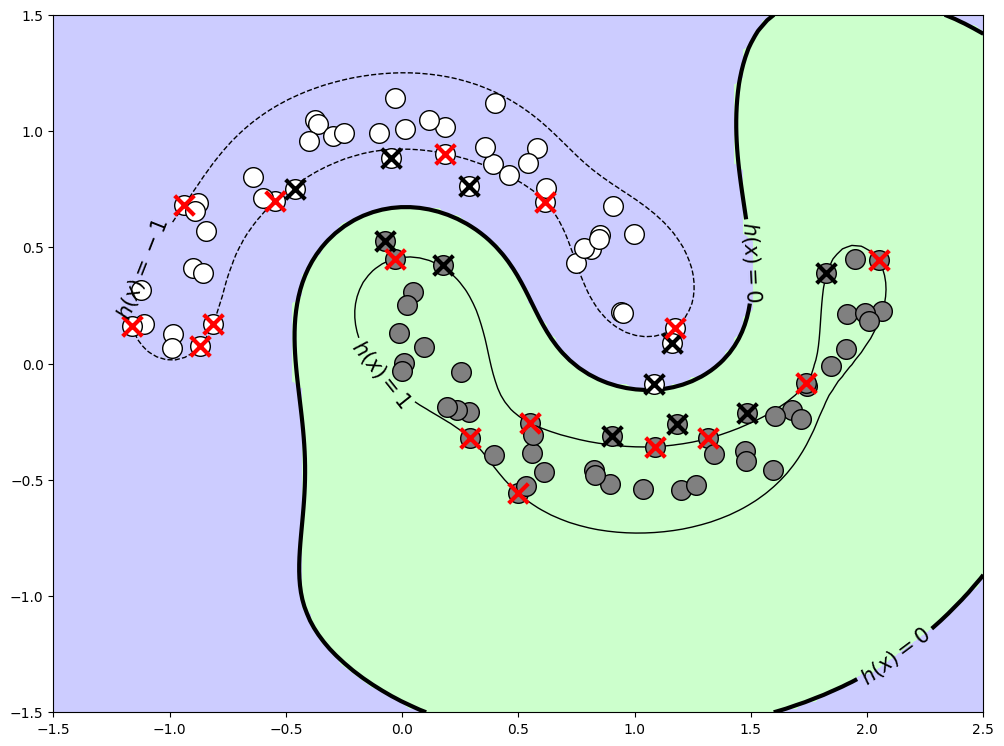
\includegraphics[width=\columnwidth]{csvc001.png}

				The support vectors are the samples indicated with a cross. A red cross indicates the samples on the margin. A black cross indicates the samples with non null slack variables $\xi$. Only the support vectors (i.e. the samples indicated with a cross) contribute to the definition of the separator.
			
\section*{C-SVC examples}


		\end{multicols*}
		\end{document}
